\chapter{Modelos de Iluminação}

Simular como a luz interage com as superfícies é o que transforma formas geométricas planas em objetos que parecem ter volume, textura e realismo. A iluminação em computação gráfica é um campo interdisciplinar que transita entre a física óptica rigorosa, a geometria diferencial e aproximações matemáticas eficientes para processamento em tempo real. Como define \textcite{shirley2021fundamentals}, o objetivo primordial de um modelo de iluminação é aproximar a radiância que chega ao observador a partir de cada ponto visível na cena. A luz não é apenas uma cor aplicada a um triângulo, mas uma entidade física que transporta energia e interage de formas complexas com a matéria através de fenômenos de absorção, reflexão, refração e espalhamento.

\section{Radiometria Básica para Gráficos}

Para compreender os modelos de iluminação modernos e o render fotorrealista, precisamos de uma base sólida em radiometria, a ciência que mede a radiação eletromagnética em termos de energia. Em computação gráfica, abstraímos o espectro contínuo de luz em três canais discretos (RGB), mas as leis físicas subjacentes permanecem as mesmas. Focamos em quatro grandezas fundamentais:

\begin{itemize}
    \item \textbf{Fluxo Radiante ($\Phi$):} Representa a energia total emitida, refletida, transmitida ou recebida por unidade de tempo por uma fonte de luz. A unidade no Sistema Internacional é o Watt (W). Em um motor de renderização, o fluxo radiante de uma lâmpada define sua potência total de emissão em todas as direções.
    \item \textbf{Irradiância ($E$):} Define a densidade de fluxo radiante que atinge uma superfície por unidade de área. Matematicamente, $E = d\Phi / dA$, medida em Watts por metro quadrado ($W/m^2$). É a irradiância que determina quão "acesa" uma superfície está antes de considerarmos o ângulo de visualização ou as propriedades do material.
    \item \textbf{Intensidade Radiante ($I$):} É o fluxo radiante emitido por uma fonte pontual por unidade de ângulo sólido ($W/sr$). O ângulo sólido ($\omega$) é medido em esterradianos (sr), e descreve a "abertura" de um cone de luz no espaço tridimensional. Uma esfera completa possui $4\pi$ esterradianos.
    \item \textbf{Radiância ($L$):} É a grandeza mais crítica para a computação gráfica. Ela mede o fluxo por unidade de ângulo sólido e por unidade de área projetada ($W/(sr \cdot m^2)$). A radiância é o que efetivamente "atravessa" o espaço e atinge um sensor de câmera ou a retina humana. Um dos princípios fundamentais da óptica geométrica é que a radiância permanece constante ao longo de um raio no vácuo, o que facilita enormemente o cálculo de visibilidade.
\end{itemize}

A relação geométrica fundamental entre irradiância e radiância em uma superfície é dada pela lei do cosseno de Lambert: $dE = L \cos\theta d\omega$. Esta relação explica por que superfícies inclinadas em relação à fonte de luz recebem menos energia e, portanto, parecem mais escuras do que superfícies perpendiculares ao feixe luminoso.

\section{Iluminação Local vs. Global}

Antes de mergulharmos nas fórmulas matemáticas, é crucial distinguir duas abordagens fundamentais que definem a complexidade e o custo computacional de um renderizador moderno:

\begin{itemize}
    \item \textbf{Iluminação Local:} Esta abordagem considera apenas a luz que viaja diretamente de uma fonte de luz (como uma lâmpada ou o sol) para um ponto específico na superfície do objeto. É extremamente rápida e eficiente, sendo o padrão para motores de jogo por décadas. No entanto, ela possui uma limitação severa: ignora o fato de que a luz reflete de um objeto para outro (interreflexão). Sem luz indireta, as áreas de sombra tornam-se pretas puras e a cena perde o realismo natural e a profundidade visual que nossos olhos esperam ver.
    \item \textbf{Iluminação Global (GI):} Simula todas as interações da luz na cena, incluindo reflexões múltiplas (\textit{bounce light}). Fenômenos como o \textit{color bleeding}, onde uma parede vermelha reflete luz avermelhada em um teto branco próximo, são capturados apenas através de modelos de GI. Algoritmos como \textit{Path Tracing}, \textit{Photon Mapping} e \textit{Radiosity} são os pilares da iluminação global. Como observa \textcite{akenine2018realtime}, a evolução do hardware, como as GPUs com núcleos dedicados a Ray Tracing, está permitindo que essas técnicas saiam do cinema e entrem nos jogos em tempo real.
\end{itemize}

\section{Tipos de Fontes de Luz e Modelos de Atenuação}

Na computação gráfica, não simulamos filamentos de tungstênio ou reações nucleares estelares de forma direta. Em vez disso, abstraímos fontes de luz físicas em modelos matemáticos simplificados:

\begin{enumerate}
    \item \textbf{Luz Direcional:} Simula fontes infinitamente distantes, como o Sol. Consideramos que todos os raios que atingem a cena são perfeitamente paralelos entre si. Devido à distância extrema, não há atenuação perceptível pela distância percorrida, apenas uma direção constante $\hat{\mathbf{l}}$ e uma intensidade de cor definida.
    \item \textbf{Luz Pontual (\textit{Point Light}):} Emitida em todas as direções a partir de um ponto infinitesimal no espaço. Na física real, a intensidade decai com o inverso do quadrado da distância ($1/d^2$). No entanto, em implementações de software, usamos uma fórmula mais flexível para evitar divisões por zero e permitir maior controle artístico:
    \begin{equation}
        I(d) = \frac{I_0}{k_c + k_l d + k_q d^2}
    \end{equation}
    Onde $k_c$ é a constante de sustentação (evita explosão de luz próxima ao ponto), $k_l$ o coeficiente linear e $k_q$ o coeficiente quadrático para uma queda mais rápida.
    \item \textbf{Luz de Holofote (\textit{Spotlight}):} Emitida dentro de um cone de influência. Além da atenuação por distância, a intensidade decai suavemente conforme o ângulo do raio se afasta do eixo central do cone. Usamos geralmente uma função de interpolação suave (\texttt{smoothstep}) entre um cone interno (brilho total) e um cone externo (escuridão total).
    \item \textbf{Luz de Área:} Emitida por superfícies geométricas reais (como um painel de LED retangular). São fundamentais para produzir sombras suaves com penumbras realistas e reflexos alongados em superfícies polidas. A técnica moderna \textbf{LTC} (\textit{Linearly Transformed Cosines}) permite calcular a iluminação de fontes poligonais de forma analítica e eficiente, integrando a BRDF sobre a área da luz sem a necessidade de amostragem estocástica pesada em tempo real.
\end{enumerate}

\section{O Modelo de Phong e sua Derivação Geométrica}

Proposto em 1975 por Bui Tuong Phong \cite{phong1975illumination}, este modelo foi a espinha dorsal da computação gráfica por gerações. Ele é um modelo fenomenológico, o que significa que ele imita a aparência das coisas sem necessariamente seguir as leis rigorosas da física. O modelo decompõe a luz em três componentes independentes: ambiente, difusa e especular.

\subsection{A Base: Lei de Lambert e Reflexão Difusa}

A derivação começa com a observação de Johann Heinrich Lambert em 1760. Superfícies ideais (Lambertianas) dispersam a luz uniformemente em todas as direções da hemisfera. A quantidade de luz que efetivamente atinge a superfície depende do ângulo de incidência $\theta$ entre a normal da superfície $\hat{\mathbf{n}}$ e o vetor da luz $\hat{\mathbf{l}}$.

\begin{formula}{Reflexão Difusa (Lambert)}
    I_d = k_d \cdot L_d \cdot \cos(\theta) = k_d \cdot L_d \cdot (\hat{\mathbf{n}} \cdot \hat{\mathbf{l}})
\end{formula}

O produto escalar $\hat{\mathbf{n}} \cdot \hat{\mathbf{l}}$ nos fornece o cosseno de forma extremamente eficiente para o hardware. Em implementações reais, usamos sempre \texttt{max(dot(n, l), 0.0)} para evitar artefatos de iluminação negativa em superfícies opostas à luz.

\subsection{A Extensão Especular e o Vetor de Reflexão}

Phong percebeu que materiais polidos exibem um brilho concentrado (\textit{specular highlight}) baseado na direção de reflexão perfeita $\hat{\mathbf{r}}$. Geometricamente, se a luz incide com um ângulo $\theta$ em relação à normal, ela reflete com o mesmo ângulo $\theta$ do lado oposto da normal, no mesmo plano definido pelos vetores incidentes.

\begin{center}
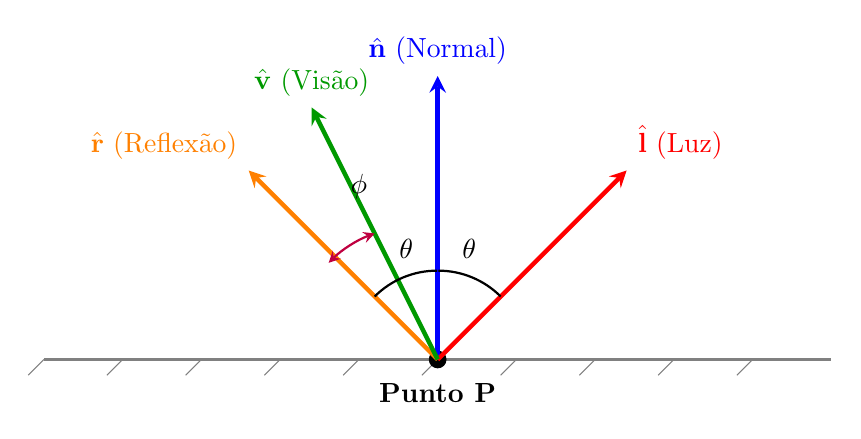
\begin{tikzpicture}[scale=2, >=stealth]
    % Surface
    \draw[thick, gray] (-2.5,0) -- (2.5,0);
    \foreach \x in {-2.5,-2.0,...,2.0}
        \draw[gray] (\x,0) -- (\x-0.1,-0.1);
    
    % Point P
    \filldraw (0,0) circle (1.5pt) node[below=5pt] {\textbf{Punto P}};
    
    % Vectors
    \draw[->, ultra thick, blue] (0,0) -- (0,1.8) node[above] {$\hat{\mathbf{n}}$ (Normal)};
    \draw[->, ultra thick, red] (0,0) -- (1.2,1.2) node[above right] {$\hat{\mathbf{l}}$ (Luz)};
    \draw[->, ultra thick, orange] (0,0) -- (-1.2,1.2) node[above left] {$\hat{\mathbf{r}}$ (Reflexão)};
    \draw[->, ultra thick, green!60!black] (0,0) -- (-0.8,1.6) node[above] {$\hat{\mathbf{v}}$ (Visão)};
    
    % Angles
    \draw[thick] (0.4,0.4) arc (45:90:0.56);
    \node at (0.2,0.7) {$\theta$};
    \draw[thick] (-0.4,0.4) arc (135:90:0.56);
    \node at (-0.2,0.7) {$\theta$};
    \draw[thick, <->, purple] (-0.4,0.8) arc (110:135:0.8);
    \node at (-0.5,1.1) {$\phi$};
\end{tikzpicture}
\end{center}

O vetor de reflexão é calculado algebricamente como $\hat{\mathbf{r}} = 2(\hat{\mathbf{n}} \cdot \hat{\mathbf{l}})\hat{\mathbf{n}} - \hat{\mathbf{l}}$. A intensidade especular de Phong é proporcional ao cosseno do ângulo $\phi$ entre o reflexo e o observador, elevado a uma potência de polidez $n$:

\begin{formula}{Reflexão Especular de Phong}
    I_s = k_s \cdot L_s \cdot (\hat{\mathbf{r}} \cdot \hat{\mathbf{v}})^n
\end{formula}

O expoente $n$ define quão "espalhado" ou "concentrado" é o brilho. Valores baixos (5-10) simulam plásticos foscos, enquanto valores altos (200-1000) simulam metais polidos ou espelhos.

\section{Blinn-Phong e o Vetor Halfway: Uma Evolução Necessária}

James Blinn em 1977 refinou o modelo de Phong para resolver problemas de performance e inconsistências visuais em ângulos rasantes. Em vez de calcular o caro vetor de reflexão $\hat{\mathbf{r}}$, ele introduziu o vetor médio (\textit{halfway vector}) $\hat{\mathbf{h}}$, que é a bissetriz exata entre o vetor da luz e o do observador:

\begin{equation}
    \hat{\mathbf{h}} = \frac{\hat{\mathbf{l}} + \hat{\mathbf{v}}}{\|\hat{\mathbf{l}} + \hat{\mathbf{v}}\|}
\end{equation}

A componente especular passa a ser calculada como $(\hat{\mathbf{n}} \cdot \hat{\mathbf{h}})^n$. Esta técnica é computacionalmente vantajosa porque o vetor $\hat{\mathbf{h}}$ pode ser considerado constante se a luz e a câmera estiverem "no infinito", economizando milhares de operações por frame em cada fragmento renderizado.

\section{A Equação de Renderização: O Coração do Fotorrealismo}

A base teórica de toda a computação gráfica moderna é a Equação de Renderização, formalizada por James Kajiya em 1986 \cite{kajiya1986rendering}. Ela descreve matematicamente o equilíbrio de energia luminosa em uma cena fechada:

\begin{equation}
    L_o(p, \omega_o) = L_e(p, \omega_o) + \int_{\Omega} f_r(p, \omega_i, \omega_o) L_i(p, \omega_i) (\hat{\mathbf{n}} \cdot \omega_i) d\omega_i
\end{equation}

Nesta equação, $L_o$ é a radiância de saída, $L_e$ é a emitida, e a integral soma toda a luz incidente refletida pela função $f_r$, conhecida como BRDF. Para ser fisicamente válida, a BRDF deve cumprir:
\begin{enumerate}
    \item \textbf{Reciprocidade de Helmholtz:} A função deve ser simétrica em relação aos raios de entrada e saída.
    \item \textbf{Conservação de Energia:} A energia total refletida não pode exceder a incidente.
\end{enumerate}

\section{Modelo de Microfacetas: A Teoria Cook-Torrance}

O \textit{Physically Based Rendering} (PBR) baseia-se na teoria das microfacetas. Assumimos que, em nível microscópico, nenhuma superfície é perfeitamente lisa, mas composta por uma infinidade de minúsculos espelhos ideais orientados de forma estocástica. O modelo de Cook-Torrance \cite{cook1982reflectance} expressa a BRDF como:

\begin{equation}
    f_r = \frac{k_d}{\pi} + \frac{D \cdot F \cdot G}{4(\hat{\mathbf{n}}\cdot\hat{\mathbf{l}})(\hat{\mathbf{n}}\cdot\hat{\mathbf{v}})}
\end{equation}

Cada termo matemático no numerador representa um fenômeno óptico distinto:

\subsection{Distribuição de Normais (D)}
A função de distribuição (NDF) define qual fração das microfacetas está orientada para refletir luz na direção do observador. O modelo GGX (Trowbridge-Reitz) tornou-se o padrão industrial por suas "caudas longas" que criam halos de brilho realistas:
\begin{equation}
    D_{GGX}(\hat{\mathbf{n}}, \hat{\mathbf{h}}, \alpha) = \frac{\alpha^2}{\pi((\hat{\mathbf{n}}\cdot\hat{\mathbf{h}})^2(\alpha^2-1)+1)^2}
\end{equation}

\subsection{O Termo de Fresnel (F)}
Descreve como a refletividade aumenta drasticamente em ângulos rasantes. Usamos a aproximação de Schlick para evitar o cálculo caro das equações de Fresnel complexas:
\begin{equation}
    F(\theta) = F_0 + (1-F_0)(1-\cos\theta)^5
\end{equation}
Metais possuem $F_0$ colorido e alto, enquanto dielétricos (plástico, madeira, vidro) possuem $F_0$ baixo, tipicamente fixado em 0.04 (4\%).

\subsection{A Função de Geometria (G)}
Este termo modela a perda de energia causada por microfacetas que bloqueiam a luz incidente (\textit{shadowing}) ou que impedem que o reflexo chegue ao observador (\textit{masking}). Sem este termo, os objetos pareceriam brilhar artificialmente nas suas silhuetas.

\section{Propriedades Avançadas de Materiais e Superfícies}

Materiais reais no mundo físico exibem comportamentos que vão muito além do modelo metálico-rugosidade simplificado:

\begin{itemize}
    \item \textbf{Anisotropia:} Simula materiais com ranhuras microscópicas orientadas (como metal escovado, cabelos ou fios de tecido). Os reflexos tornam-se alongados e perpendiculares à direção das ranhuras.
    \item \textbf{Clear Coat:} Adiciona uma segunda camada especular transparente sobre o material base (comum em verniz de madeira ou pintura de carros de luxo). Esta camada tem sua própria rugosidade e índice de refração.
    \item \textbf{Sheen:} Modela o brilho suave nas bordas de tecidos (\textit{cloth rendering}), focado no espalhamento de luz em micro-fibras, comum em veludo ou seda.
    \item \textbf{Iridescência:} Fenômeno de interferência em filmes finos onde a cor varia com o ângulo de visão e a espessura da camada (bolhas de sabão, manchas de óleo em poças).
\end{itemize}

\section{Modelos de Subsurface Scattering (SSS)}

Materiais orgânicos e translúcidos (pele humana, mármore, leite, jade) não são perfeitamente opacos. A luz penetra na superfície, viaja pelo interior sofrendo múltiplas colisões com as partículas internas e sai em pontos e direções diferentes da incidência original. Este fenômeno é conhecido como SSS. Em tempo real, técnicas como \textit{Screen-Space Subsurface Scattering} (SSSS) aplicam filtros de desfoque cromático seletivos, simulando como a luz vermelha penetra mais profundamente nos tecidos humanos do que a luz azul, dando o aspecto "vibrante" e orgânico à pele.

\section{Image-Based Lighting (IBL) e Render HDR}

Para que materiais PBR pareçam realmente integrados ao mundo virtual, eles precisam refletir o ambiente completo, não apenas luzes pontuais. O IBL utiliza mapas de cubos HDR (\textit{High Dynamic Range}) para iluminar a cena:
\begin{itemize}
    \item \textbf{Mapa de Irradiância:} Fornece a componente difusa vinda de todas as direções de forma borrada.
    \item \textbf{Mapas de Reflexão Pré-filtrados:} Fornecem reflexos especulares com diferentes níveis de nitidez baseados na rugosidade do material.
\end{itemize}

\section{Implementação PBR Completa em GLSL}

Abaixo, apresentamos uma implementação robusta do modelo de Cook-Torrance seguindo o fluxo de trabalho moderno.

\begin{lstlisting}[language=GLSL, caption={Fragment Shader PBR Completo}]
const float PI = 3.14159265359;

// Distribuição de Normais GGX
float DistributionGGX(vec3 N, vec3 H, float roughness) {
    float a = roughness * roughness;
    float a2 = a * a;
    float NdotH = max(dot(N, H), 0.0);
    float NdotH2 = NdotH * NdotH;
    float num = a2;
    float denom = (NdotH2 * (a2 - 1.0) + 1.0);
    denom = PI * denom * denom;
    return num / denom;
}

// Geometria de Schlick-GGX
float GeometrySchlickGGX(float NdotV, float roughness) {
    float r = (roughness + 1.0);
    float k = (r * r) / 8.0;
    float num = NdotV;
    float denom = NdotV * (1.0 - k) + k;
    return num / denom;
}

// Função de Geometria de Smith
float GeometrySmith(vec3 N, vec3 V, vec3 L, float roughness) {
    float NdotV = max(dot(N, V), 0.0);
    float NdotL = max(dot(N, L), 0.0);
    float ggx2 = GeometrySchlickGGX(NdotV, roughness);
    float ggx1 = GeometrySchlickGGX(NdotL, roughness);
    return ggx1 * ggx2;
}

// Fresnel-Schlick
vec3 fresnelSchlick(float cosTheta, vec3 F0) {
    return F0 + (1.0 - F0) * pow(clamp(1.0 - cosTheta, 0.0, 1.0), 5.0);
}

void main() {
    vec3 N = normalize(Normal);
    vec3 V = normalize(viewPos - FragPos);
    vec3 F0 = mix(vec3(0.04), albedo, metallic);

    vec3 Lo = vec3(0.0);
    for(int i = 0; i < numLights; ++i) {
        vec3 L = normalize(lightPositions[i] - FragPos);
        vec3 H = normalize(V + L);
        float distance = length(lightPositions[i] - FragPos);
        float attenuation = 1.0 / (distance * distance);
        vec3 radiance = lightColors[i] * attenuation;

        float D = DistributionGGX(N, H, roughness);   
        float G = GeometrySmith(N, V, L, roughness);      
        vec3 F  = fresnelSchlick(max(dot(H, V), 0.0), F0);
        
        vec3 kS = F;
        vec3 kD = (vec3(1.0) - kS) * (1.0 - metallic);
        
        vec3 numerator = D * G * F;
        float denominator = 4.0 * max(dot(N, V), 0.0) * max(dot(N, L), 0.0) + 0.0001;
        vec3 specular = numerator / denominator;
            
        float NdotL = max(dot(N, L), 0.0);                
        Lo += (kD * albedo / PI + specular) * radiance * NdotL;
    }
    
    // Tone mapping e Gamma Correction
    vec3 color = Lo / (Lo + vec3(1.0));
    color = pow(color, vec3(1.0/2.2));
    FragColor = vec4(color, 1.0);
}
\end{lstlisting}

\section*{Exercícios de Consolidação}

\begin{enumerate}
    \item \textbf{Derivação de Vetores:} Prove matematicamente que $\hat{\mathbf{r}} = 2(\hat{\mathbf{n}} \cdot \hat{\mathbf{l}})\hat{\mathbf{n}} - \hat{\mathbf{l}}$.
    \item \textbf{Conservação de Energia:} Demonstre um caso onde o modelo de Phong clássico cria energia "do nada".
    \item \textbf{Reciprocidade de Helmholtz:} Por que esta propriedade é vital para o Path Tracing bidirecional?
    \item \textbf{Atenuação Física:} Derive a lei do inverso do quadrado a partir do fluxo de uma esfera radiante.
    \item \textbf{GGX vs Blinn:} Por que o GGX possui reflexos mais realistas em materiais rugosos?
    \item \textbf{Fresnel em Metais:} Explique por que metais possuem refletividade normal ($F_0$) colorida.
    \item \textbf{Sombreamento vs Mascaramento:} Qual a diferença física entre esses dois termos da função $G$?
    \item \textbf{Subsurface Scattering:} Como a cor da luz muda ao atravessar o interior de uma mão humana?
    \item \textbf{Integração de Monte Carlo:} Como reduzir o ruído em um renderizador PBR sem aumentar o tempo de render?
    \item \textbf{Luzes de Área:} Qual a vantagem da técnica LTC sobre a amostragem de pontos tradicional?
    \item \textbf{Iridescência:} Onde podemos encontrar este fenômeno em materiais do cotidiano?
    \item \textbf{Anisotropia:} Como definir os eixos tangentes em uma malha para reflexos anisotrópicos?
    \item \textbf{Clear Coat:} Por que esta técnica exige um segundo passe de iluminação especular?
    \item \textbf{Normalização:} Por que o termo difuso da BRDF deve ser dividido por $\pi$?
    \item \textbf{Tone Mapping:} Qual a diferença entre mapeamento linear e o padrão cinematográfico ACES?
    \item \textbf{Microfacetas:} Explique o conceito de "micro-espelhos ideais" na teoria de Cook-Torrance.
    \item \textbf{Espaço de Cor:} Por que devemos converter texturas sRGB para espaço linear antes da iluminação?
    \item \textbf{Radiometria:} Qual a diferença entre radiância e irradiância em termos de ângulo sólido?
    \item \textbf{Implementação:} Como adaptar o shader acima para suportar múltiplas fontes de luz pontuais e direcionais?
    \item \textbf{Desafio:} Escreva a fórmula completa da BRDF de Cook-Torrance e identifique cada grandeza física envolvida.
\end{enumerate}


\section{O Modelo de Phong e sua Derivação}

Proposto em 1975 por Bui Tuong Phong \cite{phong1975illumination}, este modelo foi a espinha dorsal da computação gráfica por gerações. Ele não se baseia estritamente na física, mas sim em uma observação fenomenológica. O modelo assume que a iluminação total é a soma de três componentes independentes: ambiente, difusa e especular.

\subsection{A Base: Lei de Lambert}

A derivação começa com a observação de Johann Heinrich Lambert em 1760. Superfícies ideais (Lambertianas) dispersam a luz uniformemente em todas as direções. A quantidade de luz que efetivamente atinge a superfície depende do ângulo de incidência $\theta$ entre a normal $\hat{\mathbf{n}}$ e o vetor da luz $\hat{\mathbf{l}}$.

\begin{formula}{Reflexão Difusa (Lambert)}
    I_d = k_d \cdot L_d \cdot \cos(\theta) = k_d \cdot L_d \cdot (\hat{\mathbf{n}} \cdot \hat{\mathbf{l}})
\end{formula}

O produto escalar $\hat{\mathbf{n}} \cdot \hat{\mathbf{l}}$ nos fornece o cosseno de forma eficiente. Em implementações GLSL, usamos \texttt{max(dot(n, l), 0.0)} para garantir que luz vinda de "trás" da superfície não gere cores negativas.

\subsection{A Extensão Especular e o Vetor de Reflexão}

Phong percebeu que materiais polidos exibem um brilho concentrado (\textit{specular highlight}) baseado na direção de reflexão perfeita $\hat{\mathbf{r}}$. Geometricamente, se a luz incide com um ângulo $\theta$ em relação à normal, ela reflete com o mesmo ângulo $\theta$ do lado oposto.

\begin{center}
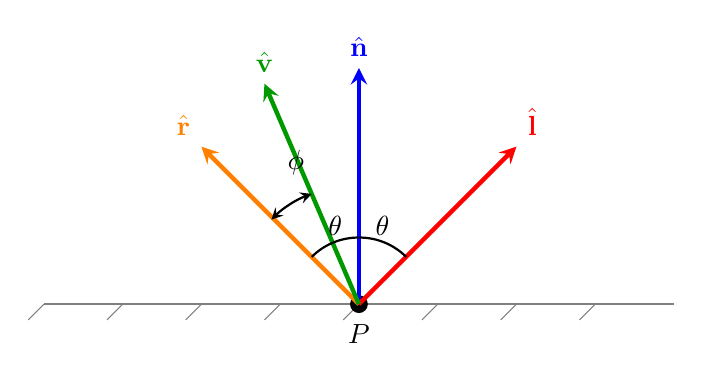
\begin{tikzpicture}[scale=2, >=stealth]
    % Surface
    \draw[thick, gray] (-2,0) -- (2,0);
    \foreach \x in {-2,-1.5,...,1.5}
        \draw[gray] (\x,0) -- (\x-0.1,-0.1);
    
    % Point P
    \filldraw (0,0) circle (1.5pt) node[below=4pt] {$P$};
    
    % Vectors
    \draw[->, ultra thick, blue] (0,0) -- (0,1.5) node[above] {$\hat{\mathbf{n}}$};
    \draw[->, ultra thick, red] (0,0) -- (1,1) node[above right] {$\hat{\mathbf{l}}$};
    \draw[->, ultra thick, orange] (0,0) -- (-1,1) node[above left] {$\hat{\mathbf{r}}$};
    \draw[->, ultra thick, green!60!black] (0,0) -- (-0.6,1.4) node[above] {$\hat{\mathbf{v}}$};
    
    % Angles
    \draw[thick] (0.3,0.3) arc (45:90:0.42);
    \node at (0.15,0.5) {$\theta$};
    \draw[thick] (-0.3,0.3) arc (135:90:0.42);
    \node at (-0.15,0.5) {$\theta$};
    \draw[thick, <->] (-0.3,0.7) arc (110:135:0.7);
    \node at (-0.4,0.9) {$\phi$};
\end{tikzpicture}
\end{center}

O vetor de reflexão é calculado como $\hat{\mathbf{r}} = 2(\hat{\mathbf{n}} \cdot \hat{\mathbf{l}})\hat{\mathbf{n}} - \hat{\mathbf{l}}$. A intensidade especular é proporcional ao cosseno do ângulo $\phi$ entre o reflexo e o observador, elevado a uma potência $n$ que define a polidez:

\begin{formula}{Reflexão Especular de Phong}
    I_s = k_s \cdot L_s \cdot (\hat{\mathbf{r}} \cdot \hat{\mathbf{v}})^n
\end{formula}

\section{Blinn-Phong e o Vetor Halfway}

James Blinn em 1977 refinou o modelo de Phong para melhorar a eficiência computacional e a qualidade visual em ângulos rasantes. Em vez de calcular o caro vetor de reflexão $\hat{\mathbf{r}}$, ele introduziu o vetor médio (\textit{halfway vector}) $\hat{\mathbf{h}}$, que é a bissetriz exata entre o vetor da luz e o do observador:

\begin{equation}
    \hat{\mathbf{h}} = \frac{\hat{\mathbf{l}} + \hat{\mathbf{v}}}{\|\hat{\mathbf{l}} + \hat{\mathbf{v}}\|}
\end{equation}

A componente especular passa a ser $(\hat{\mathbf{n}} \cdot \hat{\mathbf{h}})^n$. Esta técnica é computacionalmente vantajosa pois o vetor $\hat{\mathbf{h}}$ pode ser pré-calculado por vértice ou considerado constante se a luz e a câmera estiverem no infinito, economizando ciclos de processamento no fragment shader.

\section{A Equação de Renderização e a BRDF}

A base teórica de toda a computação gráfica moderna fotorrealista é a Equação de Renderização, formalizada por James Kajiya em 1986 \cite{kajiya1986rendering}. Ela descreve matematicamente o equilíbrio de energia luminosa em uma cena fechada:

\begin{equation}
    L_o(p, \omega_o) = L_e(p, \omega_o) + \int_{\Omega} f_r(p, \omega_i, \omega_o) L_i(p, \omega_i) (\hat{\mathbf{n}} \cdot \omega_i) d\omega_i
\end{equation}

Neste formalismo, $L_o$ representa a radiância de saída do ponto $p$ na direção $\omega_o$, $L_e$ é a radiância emitida, e a integral soma toda a luz incidente $L_i$ refletida pela função $f_r$.

A função $f_r$ é a \textbf{BRDF} (\textit{Bidirectional Reflectance Distribution Function}). Ela define a razão entre a radiância refletida e a irradiância incidente. Para ser fisicamente plausível, uma BRDF deve cumprir rigorosamente dois requisitos fundamentais:
\begin{itemize}
    \item \textbf{Reciprocidade de Helmholtz:} A função deve ser simétrica, ou seja, $f_r(\omega_i, \omega_o) = f_r(\omega_o, \omega_i)$. O caminho da luz pode ser invertido sem alterar a proporção de reflexão.
    \item \textbf{Conservação de Energia:} A energia total que sai de uma superfície nunca pode ser maior que a energia incidente. Matematicamente, $\int_{\Omega} f_r(\omega_i, \omega_o) \cos\theta_o d\omega_o \le 1$.
\end{itemize}

\section{Modelo de Microfacetas: Teoria Completa}

O \textit{Physically Based Rendering} (PBR) baseia-se na teoria das microfacetas. Assumimos que, em nível microscópico, uma superfície não é perfeitamente lisa, mas composta por uma infinidade de minúsculos espelhos ideais orientados aleatoriamente. A rugosidade do material determina quão caótica é a distribuição dessas microfacetas. O modelo de Cook-Torrance \cite{cook1982reflectance} é a implementação matemática mais bem-sucedida dessa teoria:

\begin{equation}
    f_r = \frac{k_d}{\pi} + \frac{D \cdot F \cdot G}{4(\hat{\mathbf{n}}\cdot\hat{\mathbf{l}})(\hat{\mathbf{n}}\cdot\hat{\mathbf{v}})}
\end{equation}

Cada termo do numerador da componente especular representa um fenômeno físico distinto:

\subsection{Distribuição de Normais (D)}
A função de distribuição (NDF) define qual fração das microfacetas está orientada exatamente na direção do vetor médio $\hat{\mathbf{h}}$. O modelo GGX (Trowbridge-Reitz) é o padrão atual devido às suas "caudas longas" que criam brilhos mais naturais e suaves:
\begin{equation}
    D_{GGX}(\hat{\mathbf{n}}, \hat{\mathbf{h}}, \alpha) = \frac{\alpha^2}{\pi((\hat{\mathbf{n}}\cdot\hat{\mathbf{h}})^2(\alpha^2-1)+1)^2}
\end{equation}
Aqui, $\alpha$ representa o parâmetro de rugosidade elevada ao quadrado ($\alpha = \text{roughness}^2$).

\subsection{Termo de Fresnel (F)}
Descreve como a refletividade aumenta dramaticamente quando o ângulo de incidência se aproxima de 90 graus (ângulos rasantes). Quase todos os materiais tornam-se espelhos perfeitos em ângulos agudos. Usamos a aproximação de Schlick:
\begin{equation}
    F(\theta) = F_0 + (1-F_0)(1-\cos\theta)^5
\end{equation}
O parâmetro $F_0$ é a refletividade na incidência normal. Metais possuem $F_0$ colorido e alto, enquanto dielétricos (plástico, madeira, vidro) possuem $F_0$ baixo, em torno de 0.04.

\subsection{Função de Geometria (G)}
Modela a perda de energia devido a microfacetas que bloqueiam a luz incidente (\textit{shadowing}) ou que impedem que o reflexo chegue ao observador (\textit{masking}). Sem este termo, as bordas dos objetos pareceriam excessivamente brilhantes. A função de Smith baseada em GGX é a mais comum:
\begin{equation}
    G(\hat{\mathbf{n}}, \hat{\mathbf{v}}, \hat{\mathbf{l}}, \alpha) = G_1(\hat{\mathbf{n}}, \hat{\mathbf{v}}, \alpha) \cdot G_1(\hat{\mathbf{n}}, \hat{\mathbf{l}}, \alpha)
\end{equation}

\section{Propriedades Avançadas de Materiais}

Para além do modelo metálico-rugosidade básico, materiais reais exibem comportamentos mais complexos que exigem extensões na BRDF:

\begin{itemize}
    \item \textbf{Anisotropia:} Simula materiais com ranhuras microscópicas orientadas (como metal escovado, cabelos ou discos de vinil). Os reflexos tornam-se alongados e perpendiculares à direção das ranhuras.
    \item \textbf{Clear Coat:} Adiciona uma segunda camada especular transparente sobre o material base (comum em pintura automotiva). Esta camada possui sua própria rugosidade e índice de refração, exigindo um cálculo de Fresnel adicional para atenuar a luz que penetra na camada inferior.
    \item \textbf{Sheen:} Modela o brilho suave nas bordas de tecidos (\textit{cloth rendering}), focando no espalhamento de luz em fibras microscópicas, comum em veludo ou cetim.
    \item \textbf{Iridescência:} Fenômeno de interferência em filmes finos onde a cor varia com o ângulo de visão e a espessura da camada superficial (bolhas de sabão, manchas de óleo).
\end{itemize}

\section{Modelos de Subsurface Scattering (SSS)}

Materiais orgânicos e translúcidos (pele humana, mármore, leite, cera) não são perfeitamente opacos. A luz penetra na superfície, viaja pelo interior sofrendo colisões e sai em pontos e direções diferentes. Este fenômeno é o SSS. O modelo clássico é o de Dipolo. Em tempo real, técnicas de \textit{Screen-Space Subsurface Scattering} (SSSS) aplicam filtros de desfoque cromático no buffer de imagem, simulando como a luz vermelha penetra mais profundamente nos tecidos humanos do que a luz azul, dando o aspecto "vivo" à pele.

\section{Image-Based Lighting (IBL) e Radiância de Ambiente}

Para que materiais PBR pareçam integrados, eles devem refletir o ambiente completo. O IBL utiliza mapas de cubos HDR para iluminar a cena. A componente difusa usa um mapa de irradiância (altamente borrado), enquanto a especular usa mapas de reflexão pré-filtrados com diferentes níveis de rugosidade (\textit{Prefiltered Environment Maps}), permitindo simular reflexos nítidos ou borrados de forma eficiente.

\section{Amostragem de Importância e Integração de Monte Carlo}

Em renderizadores modernos (Path Tracers), usamos a \textbf{Integração de Monte Carlo} para estimar o valor da Equação de Renderização sorteando direções aleatórias. Para reduzir o ruído visual, usamos a \textbf{Amostragem de Importância} (\textit{Importance Sampling}), onde sorteamos mais raios em direções onde a BRDF é maior (próximo ao reflexo especular), acelerando drasticamente a convergência da imagem.

\section{Implementação PBR Completa em GLSL}

Abaixo, apresentamos uma implementação robusta do modelo de Cook-Torrance seguindo o fluxo de trabalho moderno de rugosidade e metalicidade.

\begin{lstlisting}[language=GLSL, caption={Fragment Shader PBR Completo}]
const float PI = 3.14159265359;

// Distribuição de Normais GGX
float DistributionGGX(vec3 N, vec3 H, float roughness) {
    float a = roughness * roughness;
    float a2 = a * a;
    float NdotH = max(dot(N, H), 0.0);
    float NdotH2 = NdotH * NdotH;
    float num = a2;
    float denom = (NdotH2 * (a2 - 1.0) + 1.0);
    denom = PI * denom * denom;
    return num / denom;
}

// Geometria de Schlick-GGX para um único vetor
float GeometrySchlickGGX(float NdotV, float roughness) {
    float r = (roughness + 1.0);
    float k = (r * r) / 8.0;
    float num = NdotV;
    float denom = NdotV * (1.0 - k) + k;
    return num / denom;
}

// Função de Geometria de Smith: combina Shadowing e Masking
float GeometrySmith(vec3 N, vec3 V, vec3 L, float roughness) {
    float NdotV = max(dot(N, V), 0.0);
    float NdotL = max(dot(N, L), 0.0);
    float ggx2 = GeometrySchlickGGX(NdotV, roughness);
    float ggx1 = GeometrySchlickGGX(NdotL, roughness);
    return ggx1 * ggx2;
}

// Equação de Fresnel-Schlick para refletividade angular
vec3 fresnelSchlick(float cosTheta, vec3 F0) {
    return F0 + (1.0 - F0) * pow(clamp(1.0 - cosTheta, 0.0, 1.0), 5.0);
}

void main() {
    vec3 N = normalize(Normal);
    vec3 V = normalize(viewPos - FragPos);
    
    // F0 para dielétricos comuns é 0.04. Para metais, usamos o albedo.
    vec3 F0 = mix(vec3(0.04), albedo, metallic);

    vec3 Lo = vec3(0.0);
    for(int i = 0; i < numLights; ++i) {
        vec3 L = normalize(lightPositions[i] - FragPos);
        vec3 H = normalize(V + L);
        float distance = length(lightPositions[i] - FragPos);
        float attenuation = 1.0 / (distance * distance);
        vec3 radiance = lightColors[i] * attenuation;

        // Cálculo dos termos da BRDF
        float D = DistributionGGX(N, H, roughness);   
        float G = GeometrySmith(N, V, L, roughness);      
        vec3 F  = fresnelSchlick(max(dot(H, V), 0.0), F0);
        
        vec3 kS = F;
        vec3 kD = (vec3(1.0) - kS) * (1.0 - metallic);
        
        vec3 numerator = D * G * F;
        float denominator = 4.0 * max(dot(N, V), 0.0) * max(dot(N, L), 0.0) + 0.0001;
        vec3 specular = numerator / denominator;
            
        float NdotL = max(dot(N, L), 0.0);                
        Lo += (kD * albedo / PI + specular) * radiance * NdotL;
    }
    
    // Tone mapping e Correção Gama essential
    vec3 color = Lo / (Lo + vec3(1.0));
    color = pow(color, vec3(1.0/2.2));
    FragColor = vec4(color, 1.0);
}
\end{lstlisting}

\section*{Exercícios de Consolidação}

\begin{enumerate}
    \item \textbf{Dedução Vetorial:} Prove algebricamente que $\hat{\mathbf{r}} = 2(\hat{\mathbf{n}} \cdot \hat{\mathbf{l}})\hat{\mathbf{n}} - \hat{\mathbf{l}}$. Use a projeção de $\hat{\mathbf{l}}$ sobre a normal.
    \item \textbf{Conservação de Energia:} Explique por que o modelo de Phong clássico pode refletir mais luz do que recebe e como o modelo de Cook-Torrance resolve isso matematicamente.
    \item \textbf{Reciprocidade:} Descreva um cenário de renderização onde a Reciprocidade de Helmholtz é violada por um erro de implementação e as consequências visuais disso.
    \item \textbf{Atenuação Física:} Demonstre que a irradiância de uma luz pontual decai com $1/d^2$ utilizando o conceito de conservação de fluxo através de uma esfera.
    \item \textbf{GGX vs Phong:} Analise visualmente a diferença entre a função GGX e o modelo especular de Phong. Por que o GGX é considerado superior para metais?
    \item \textbf{Fresnel e Metais:} Por que o parâmetro $F_0$ é colorido para metais como ouro e cobre, enquanto é monocromático para plásticos?
    \item \textbf{Geometria:} Explique a diferença física entre \textit{shadowing} (sombreamento) e \textit{masking} (mascaramento) em uma superfície de microfacetas.
    \item \textbf{Subsurface Scattering:} Como o parâmetro de "espessura" influencia a cor final de um objeto translúcido em um shader de SSS?
    \item \textbf{Amostragem de Monte Carlo:} Por que não usamos amostragem puramente uniforme para integrar a BRDF em um renderizador moderno?
    \item \textbf{Luzes de Área:} Qual a vantagem da técnica de LTC (\textit{Linearly Transformed Cosines}) sobre a amostragem por pontos (\textit{Next Event Estimation})?
    \item \textbf{Iridescência:} Como a espessura de um filme fino afeta as cores observadas através do fenômeno de interferência?
    \item \textbf{Anisotropia:} Desenhe os vetores tangentes necessários para calcular a BRDF de um material anisotrópico.
    \item \textbf{Clear Coat:} Por que a luz que atinge a camada base de um material com verniz deve ser atenuada pelo termo de Fresnel da camada superior?
    \item \textbf{Normalização Difusa:} Demonstre matematicamente por que o fator $1/\pi$ garante que a componente difusa da BRDF conserva energia.
    \item \textbf{Tone Mapping:} Explique a diferença entre um mapeamento de tons linear e um mapeamento cinematográfico (como o ACES).
    \item \textbf{BRDF vs BSSRDF:} Pesquise e explique a diferença fundamental entre uma BRDF e uma BSSRDF no contexto de espalhamento interno.
    \item \textbf{Microfacetas e Rugosidade:} Por que o termo $1/4(\hat{\mathbf{n}}\cdot\hat{\mathbf{l}})(\hat{\mathbf{n}}\cdot\hat{\mathbf{v}})$ é necessário na BRDF de Cook-Torrance?
    \item \textbf{Lei de Lambert:} Prove que a integral da componente de Lambert sobre o hemisfério resulta em $\pi k_d$.
    \item \textbf{Materiais Condutores:} Explique por que metais não possuem componente difusa na prática.
    \item \textbf{Implementação:} Adicione suporte a \textit{Image-Based Lighting} ao fragment shader apresentado anteriormente.
\end{enumerate}

